\documentclass{article}
\usepackage[utf8]{inputenc}
\usepackage{amsmath}
\usepackage{graphicx}
\usepackage{float}
\usepackage{subcaption}
\usepackage[style=ieee, backend=biber ,citestyle=numeric-comp]{biblatex}
\usepackage{indentfirst}
\usepackage{chngcntr}
\usepackage[a4paper]{geometry}
\usepackage{fancyhdr}
\usepackage[hidelinks]{hyperref}
\usepackage{mathrsfs}
\usepackage[toc,page]{appendix}
\usepackage[longtable]{multirow}
\usepackage{longtable}
\usepackage{booktabs} % Para tablas súper pro
\usepackage{vcell}
\usepackage{array}
\usepackage{epsfig}
\usepackage{pdfpages}
\usepackage{amssymb}
\usepackage{pmboxdraw}
\usepackage{alltt}
\usepackage{listings}
\usepackage{listingsutf8}
\usepackage[spanish, es-tabla]{babel} % Para que ponga tabla en vez de cuadro
\usepackage{xcolor}
\usepackage{url}
\addbibresource{bibliography.bib}
\usepackage{svg}
\usepackage{xcolor,colortbl}
\usepackage{booktabs}
\usepackage{gensymb}
\usepackage{dirtytalk}
\usepackage{cancel} % Para tachar términos de ecuaciones
\usepackage{siunitx}
\usepackage{mathtools}
\usepackage{empheq}



\lstset{
     literate=%
         {á}{{\'a}}1
         {í}{{\'i}}1
         {é}{{\'e}}1
         {ú}{{\'u}}1
         {ó}{{\'o}}1
         {Á}{{\'A}}1
         {Í}{{\'I}}1
         {É}{{\'E}}1
         {Ú}{{\'U}}1
         {Ó}{{\'O}}1}

\definecolor{codegreen}{rgb}{0,0.6,0}
\definecolor{codegray}{rgb}{0.5,0.5,0.5}
\definecolor{codepurple}{rgb}{0.58,0,0.82}
\definecolor{backcolour}{rgb}{0.95,0.95,0.92}

\lstdefinestyle{mystyle}{
    backgroundcolor=\color{backcolour},   
    commentstyle=\color{codegreen},
    keywordstyle=\color{magenta},
    numberstyle=\tiny\color{codegray},
    stringstyle=\color{codepurple},
    basicstyle=\ttfamily\footnotesize,
    breakatwhitespace=false,         
    breaklines=true,                 
    captionpos=b,                    
    keepspaces=true,                 
    numbers=left,                    
    numbersep=5pt,                  
    showspaces=false,                
    showstringspaces=false,
    showtabs=false,                  
    tabsize=2
}
\lstset{style=mystyle}


\numberwithin{equation}{section}
\numberwithin{equation}{subsection}
\counterwithin{figure}{section}
\counterwithin{table}{section}
\AtBeginDocument{\counterwithin{lstlisting}{section}}

\renewcommand{\tablename}{Tabla}
\renewcommand{\spanishtablename}{Tabla}
\renewcommand{\figurename}{Figura}
\renewcommand{\contentsname}{Contenidos}
\renewcommand{\listfigurename}{Lista de figuras}
\renewcommand{\listtablename}{Lista de tablas}
\renewcommand{\lstlistingname}{Algoritmo}
\renewcommand{\figureautorefname}{Figura}
\renewcommand{\tableautorefname}{Tabla}
\renewcommand{\equationautorefname}{Ecuación}
\renewcommand{\sectionautorefname}{Sección}
% \renewcommand{\thesection}{Sección \Arabic{section}}


\geometry{top=3.5cm, bottom=3.5cm, left=3cm, right=3cm}

\pagestyle{fancy}
\fancyhf{}
\lhead{MUSE: Estructuras de uso espacial}
\rhead{
\includegraphics[height=0.8cm]{logomuse2}} % right logo
\cfoot{\thepage}



\begin{document}

\begin{center}
\thispagestyle{empty}


\includegraphics[width=16.5cm]{Logo_portada.png} \\

\vspace{2.5cm}

{\huge \textbf{Universidad Politécnica de Madrid}}\\
\vspace{1cm} 
{\scshape\Large Estructuras de uso Espacial \par}
\begin{center}
\vspace{3.5 cm}
{\bfseries\Huge Diseño y modelización de la estructura de un microsatélite: bandeja intermedia \par}
\vspace{7 cm}

\vfill
{\Large Autor:  \par}

{\Large Guillermo García del Río \par}

\end{center}
\end{center}

\pagenumbering{gobble}
\thispagestyle{empty}

\newpage
\pagenumbering{Roman} % Numeración romana hasta la primera sección


\tableofcontents


\listoffigures


\listoftables


\setlength{\parskip}{4mm}
\setlength{\parindent}{20pt}
\setlength{\headheight}{16.07225pt}

\newpage
\pagenumbering{arabic}

\input{1. Introducción.tex}
\section{Enunciado}

Se ha de diseñar una bandeja cuadrada que corresponda a la bandeja inferior del microsatélite. Esta bandeja tendra por tanto que soportar tanto una masa puntual correspondiente a los equipos que se sitúen sobre ella como una segunda masa que simule el peso del resto del satélite. Además, con el fin de modelizar la unión de la bandeja al sistema de separación, se han de incluir una serie de elementos \textit{CBUSH} que simulen los tornillos. Las dimensiones de la bandeja, la masa de los equipos y del satélite y la configuración de los rigidizadores interiores ha sido asignada en función del grupo de trabajo, siendo la descrita en este informe la que se muestra en la \autoref{tab: caracteristicas} y \autoref{fig: configrigi}.

\begin{table}[H]
\centering
\caption{Características de la bandeja asignada.}
\label{tab: caracteristicas}
\begin{tabular}{l c c c}
\toprule
\multicolumn{1}{c}{\textbf{Configuración}}  & \multicolumn{1}{c}{\textbf{Masa equipos} [kg]}   & \multicolumn{1}{c}{\textbf{Masa estructura} [kg]} & \multicolumn{1}{c}{\textbf{Dimensiones} [mm]} \\ \midrule
  Ortogonal ($\pm 45^{\circ}$ )  & 11 & 39.325 & 450 $\times$ 450 \\ \bottomrule
\end{tabular}
\end{table}

\begin{figure}[H]
    \centering
    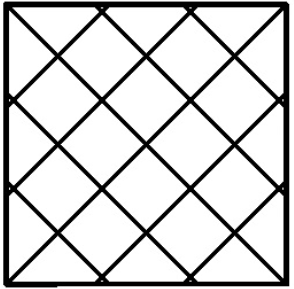
\includegraphics[scale=0.7]{Figures/Config.png}
    \caption{Configuración ortogonal $\pm 45^{\circ}$}
    \label{fig: configrigi}
\end{figure}

Las masas puntuales especificadas en la \autoref{tab: caracteristicas} han de colocarse de la siguiente forma:
\begin{itemize}
\item La masa del equipo se modeliza igual que en el caso de la bandeja intermedia, esto es, colocando una masa puntual ubicada en el eje de simetría de la bandeja, a una distancia de 80 mm sobre la superficie. Para lograr la unión entre el equipo y la bandeja, se utiliza un elemento rígido RBE2, conectados a 4 puntos de la bandeja. Los puntos de conexión en la bandeja son seleccionados por cada grupo, siendo preferible que estén en el cruce de los rigidizadores.
\item La masa del resto de la estructura se simula incluyendo una segunda masa puntual que representa la masa del resto del satélite (3 bandejas rigidizadas, 2 equipos, 4 paneles laterales y 4 vigas en L) que se apoya sobre el contorno exterior de esta bandeja inferior mediante un elemento rígido RBE2. Esta segunda masa está situada en el eje central, a una distancia de 0.38 m con respecto al plano de la bandeja
\end{itemize}

El número de elementos \textit{CBUSH} de la union adaptador-bandeja ha de oscilar entre 8 y 12, estando los nodos superiores de estos elementos situados en la bandeja y los inferiores a 20 mm de la misma. Sobre estos últimos nodos se aplican restricciones a los 6 grados de libertad 

Los requisitos estructurales que debe de cumplir el diseño propuesto se muestran en la \autoref{tab: requisitos estructurales}.

\begin{table}[H]
\centering
\caption{Requisitos estructurales de la bandeja intermedia.}
\label{tab: requisitos estructurales}
\begin{tabular}{l c}
\toprule
\multicolumn{1}{c}{\textbf{Requisitos}} & \multicolumn{1}{c}{\textbf{Valores}}\\ \midrule
 Frecuencias propias & $f_{n} > 100$ Hz \\ 
 & \\
 Márgenes de seguridad en los & \multirow{2}{*}{$MoS_{i}>0$} \\ 
 principales análisis estructurales & \\\bottomrule
\end{tabular}
\end{table}

Los análisis que se deben realizar son los siguientes:

\begin{itemize}
\item Análisis de modos propios, para el cálculo de las frecuencias propias.
\item Análisis estáticos (uno en cada eje), para el cálculo de los márgenes de seguridad de tensiones. Las aceleraciones utilizadas para los análisis estáticos en función de la dirección se muestra en la .
\end{itemize}

\begin{table}[H]
\centering
\caption{Aceleraciones en función de la dirección de aplicación.}
\label{tab: aceleraciones}      
\begin{tabular}{l c}
\toprule
\multicolumn{1}{c}{\textbf{Dirección}} & \multicolumn{1}{c}{\textbf{Aceleración} [g]}\\ \midrule
 Lateral (paralelo a la bandeja)   & 50   \\
 Longitudinal (normal a la bandeja) & 80 \\ \bottomrule
\end{tabular}
\end{table}

Para el cálculo de los márgenes de seguridad, se debe aplicar las fórmulas obtenidas de \cite{garcia2023manual}.

\begin{equation}
MoS_{y} = \left(\dfrac{\sigma_{y}}{\sigma_{\text{VMmax}} K_{p} K_{m} K_{LD} FOSY}\right)-1,
\end{equation}

\begin{equation}
    MoS_{u} = \left(\dfrac{\sigma_{u}}{\sigma_{\text{VMmax}} K_{p} K_{m} K_{LD} FOSU}\right)-1.
\end{equation}

Todos los parámetros de estas escuaciones se muestran en la \autoref{tab: paramsequs}.

\begin{table}[H]
\centering
\caption{Parámetros para el cálculo de los márgenes de seguridad.}
\label{tab: paramsequs}
\begin{tabular}{c l c}
\toprule
\multicolumn{1}{c}{\textbf{Parámetro}} & \multicolumn{1}{c}{\textbf{Significado}} & \multicolumn{1}{c}{\textbf{Valor}} \\ \midrule
  $K_{p}$   & Factor de proyecto  & 1.1 \\
  & & \\
  $K_{M}$   & Factor del modelo   & 1.2 \\
  & & \\
  $K_{LD}$  & Factor de diseño local & 1.1 \\ 
  & & \\
  $FOSY$    & Factor de seguridad del límite elástico & 1.1 \\
  & & \\ 
  $FOSU$    & Factor de seguridad de la carga última  & 1.25 \\ 
  & & \\
  $\sigma_{y}$ & Límite elástico del material & \multicolumn{1}{l}{Depende del material} \\
  & & \\ 
  $\sigma_{u}$ & Resistencia última del material & \multicolumn{1}{l}{Depende del material} \\ 
  & & \\
  \multirow{2}{*}{$\sigma_{\text{VMmax}}$ }& Máxima tensión de Von Mises obtenido & \multicolumn{1}{l}{\multirow{2}{*}{Solución de cada análisis}} \\ 
  & de un análisis determinado & \\
\bottomrule
\end{tabular}
\end{table}

Teniendo en cuenta todo lo anterior, se debe determinar el diseño óptimo de la bandeja. Las variables que se deben variar para conseguir el diseño son:

\begin{itemize}
\item Cantidad y colocación de rigidizadores interiores (respetando la configuracón mostrada en la \autoref{fig: configrigi}).
\item Material.
\item Espesor de la placa de la bandeja.
\item Dimensiones de la sección rectangular de los rigidizadores exteriores.
\item Diseño de la sección de los rigidizadores interiores y sus correspondientes dimensiones.
\end{itemize}

Como objetivo de la optimización de la bandeja intermedia, se debe conseguir cumplir con \textbf{al menos uno} de los siguientes criterios:

\begin{itemize}
\item La primera frecuencia propia se sitúe entre 100 y 125 Hz.
\item El margen de seguridad para el valor máximo de tensión de Von Mises en el \textbf{caso de carga más crítico} se sitúe entre 0 y 0.5. 
\end{itemize}
\input{3. Solución.tex}
\newpage
\section{Conclusiones}

Tras finalizar el proceso iterativo de esta bandeja se concluye que los esfuerzos que esta ha de soportar son considerablemente más elevados que en el caso de la bandeja intermedia y superior, por lo que es inviable hacerla de aluminio. Por otra parte, cabe destacar de nuevo la relevancia de la disposición y tamalo de los rigidizadores, que, tal y como se muestra en \autoref{tab:iteraciones}, permite disminuir el espesor de la bandeja según se aumenta la cantidad de rigidizadores. 



\newpage
\clearpage

\printbibliography[title = {Bibliografía}]

\newpage
\clearpage

% \appendix
% \section{Script de GMAT}

\begin{lstlisting}[language=MATLAB, caption= Scrit de GMAT]

%General Mission Analysis Tool(GMAT) Script
%Created: 2022-11-11 12:56:01


%----------------------------------------
%---------- Spacecraft
%----------------------------------------

Create Spacecraft PequeSpace;
GMAT PequeSpace.DateFormat = UTCGregorian;
GMAT PequeSpace.Epoch = '19 Aug 2014 11:59:28.000';
GMAT PequeSpace.CoordinateSystem = EarthMJ2000Eq;
GMAT PequeSpace.DisplayStateType = Keplerian;
GMAT PequeSpace.SMA = 15738;
GMAT PequeSpace.ECC = 0.5807000000000001;
GMAT PequeSpace.INC = 29.99999999999998;
GMAT PequeSpace.RAAN = 0;
GMAT PequeSpace.AOP = 0;
GMAT PequeSpace.TA = 0;
GMAT PequeSpace.DryMass = 800;
GMAT PequeSpace.Cd = 2.5;
GMAT PequeSpace.Cr = 0;
GMAT PequeSpace.DragArea = 20;
GMAT PequeSpace.SRPArea = 20;
GMAT PequeSpace.SPADDragScaleFactor = 1;
GMAT PequeSpace.SPADSRPScaleFactor = 1;
GMAT PequeSpace.Tanks = {ChemicalTank1};
GMAT PequeSpace.Thrusters = {ChemicalThruster1};
GMAT PequeSpace.NAIFId = -10002001;
GMAT PequeSpace.NAIFIdReferenceFrame = -9002001;
GMAT PequeSpace.OrbitColor = Red;
GMAT PequeSpace.TargetColor = Teal;
GMAT PequeSpace.OrbitErrorCovariance = [ 1e+70 0 0 0 0 0 ; 0 1e+70 0 0 0 0 ; 0 0 1e+70 0 0 0 ; 0 0 0 1e+70 0 0 ; 0 0 0 0 1e+70 0 ; 0 0 0 0 0 1e+70 ];
GMAT PequeSpace.CdSigma = 1e+70;
GMAT PequeSpace.CrSigma = 1e+70;
GMAT PequeSpace.Id = 'SatId';
GMAT PequeSpace.Attitude = CoordinateSystemFixed;
GMAT PequeSpace.SPADSRPInterpolationMethod = Bilinear;
GMAT PequeSpace.SPADSRPScaleFactorSigma = 1e+70;
GMAT PequeSpace.SPADDragInterpolationMethod = Bilinear;
GMAT PequeSpace.SPADDragScaleFactorSigma = 1e+70;
GMAT PequeSpace.ModelFile = 'aura.3ds';
GMAT PequeSpace.ModelOffsetX = 0;
GMAT PequeSpace.ModelOffsetY = 0;
GMAT PequeSpace.ModelOffsetZ = 0;
GMAT PequeSpace.ModelRotationX = 0;
GMAT PequeSpace.ModelRotationY = 0;
GMAT PequeSpace.ModelRotationZ = 0;
GMAT PequeSpace.ModelScale = 1;
GMAT PequeSpace.AttitudeDisplayStateType = 'Quaternion';
GMAT PequeSpace.AttitudeRateDisplayStateType = 'AngularVelocity';
GMAT PequeSpace.AttitudeCoordinateSystem = EarthMJ2000Eq;
GMAT PequeSpace.EulerAngleSequence = '321';



%----------------------------------------
%---------- Spacecraft
%----------------------------------------

Create Spacecraft FalconFoge;
GMAT FalconFoge.DateFormat = UTCGregorian;
GMAT FalconFoge.Epoch = '19 Aug 2014 11:59:28.000';
GMAT FalconFoge.CoordinateSystem = EarthMJ2000Eq;
GMAT FalconFoge.DisplayStateType = Keplerian;
GMAT FalconFoge.SMA = 15738;
GMAT FalconFoge.ECC = 0.5807000000000001;
GMAT FalconFoge.INC = 29.99999999999998;
GMAT FalconFoge.RAAN = 0;
GMAT FalconFoge.AOP = 0;
GMAT FalconFoge.TA = 0;
GMAT FalconFoge.DryMass = 800;
GMAT FalconFoge.Cd = 2.5;
GMAT FalconFoge.Cr = 0;
GMAT FalconFoge.DragArea = 20;
GMAT FalconFoge.SRPArea = 20;
GMAT FalconFoge.SPADDragScaleFactor = 1;
GMAT FalconFoge.SPADSRPScaleFactor = 1;
GMAT FalconFoge.Tanks = {ChemicalTank1};
GMAT FalconFoge.Thrusters = {ChemicalThruster1};
GMAT FalconFoge.NAIFId = -10002001;
GMAT FalconFoge.NAIFIdReferenceFrame = -9002001;
GMAT FalconFoge.OrbitColor = [0 255 0];
GMAT FalconFoge.TargetColor = Teal;
GMAT FalconFoge.OrbitErrorCovariance = [ 1e+70 0 0 0 0 0 ; 0 1e+70 0 0 0 0 ; 0 0 1e+70 0 0 0 ; 0 0 0 1e+70 0 0 ; 0 0 0 0 1e+70 0 ; 0 0 0 0 0 1e+70 ];
GMAT FalconFoge.CdSigma = 1e+70;
GMAT FalconFoge.CrSigma = 1e+70;
GMAT FalconFoge.Id = 'SatId';
GMAT FalconFoge.Attitude = CoordinateSystemFixed;
GMAT FalconFoge.SPADSRPInterpolationMethod = Bilinear;
GMAT FalconFoge.SPADSRPScaleFactorSigma = 1e+70;
GMAT FalconFoge.SPADDragInterpolationMethod = Bilinear;
GMAT FalconFoge.SPADDragScaleFactorSigma = 1e+70;
GMAT FalconFoge.ModelFile = 'aura.3ds';
GMAT FalconFoge.ModelOffsetX = 0;
GMAT FalconFoge.ModelOffsetY = 0;
GMAT FalconFoge.ModelOffsetZ = 0;
GMAT FalconFoge.ModelRotationX = 0;
GMAT FalconFoge.ModelRotationY = 0;
GMAT FalconFoge.ModelRotationZ = 0;
GMAT FalconFoge.ModelScale = 1;
GMAT FalconFoge.AttitudeDisplayStateType = 'Quaternion';
GMAT FalconFoge.AttitudeRateDisplayStateType = 'AngularVelocity';
GMAT FalconFoge.AttitudeCoordinateSystem = EarthMJ2000Eq;
GMAT FalconFoge.EulerAngleSequence = '321';

%----------------------------------------
%---------- Hardware Components
%----------------------------------------

Create ChemicalTank ChemicalTank1;
GMAT ChemicalTank1.AllowNegativeFuelMass = true;
GMAT ChemicalTank1.FuelMass = 20;
GMAT ChemicalTank1.Pressure = 1500;
GMAT ChemicalTank1.Temperature = 20;
GMAT ChemicalTank1.RefTemperature = 20;
GMAT ChemicalTank1.Volume = 0.75;
GMAT ChemicalTank1.FuelDensity = 1260;
GMAT ChemicalTank1.PressureModel = PressureRegulated;

Create ChemicalThruster ChemicalThruster1;
GMAT ChemicalThruster1.CoordinateSystem = Local;
GMAT ChemicalThruster1.Origin = Earth;
GMAT ChemicalThruster1.Axes = VNB;
GMAT ChemicalThruster1.ThrustDirection1 = 1;
GMAT ChemicalThruster1.ThrustDirection2 = 0;
GMAT ChemicalThruster1.ThrustDirection3 = 0;
GMAT ChemicalThruster1.DutyCycle = 1;
GMAT ChemicalThruster1.ThrustScaleFactor = 1;
GMAT ChemicalThruster1.DecrementMass = false;
GMAT ChemicalThruster1.GravitationalAccel = 9.81;
GMAT ChemicalThruster1.C1 = 10;
GMAT ChemicalThruster1.C2 = 0;
GMAT ChemicalThruster1.C3 = 0;
GMAT ChemicalThruster1.C4 = 0;
GMAT ChemicalThruster1.C5 = 0;
GMAT ChemicalThruster1.C6 = 0;
GMAT ChemicalThruster1.C7 = 0;
GMAT ChemicalThruster1.C8 = 0;
GMAT ChemicalThruster1.C9 = 0;
GMAT ChemicalThruster1.C10 = 0;
GMAT ChemicalThruster1.C11 = 0;
GMAT ChemicalThruster1.C12 = 0;
GMAT ChemicalThruster1.C13 = 0;
GMAT ChemicalThruster1.C14 = 0;
GMAT ChemicalThruster1.C15 = 0;
GMAT ChemicalThruster1.C16 = 0;
GMAT ChemicalThruster1.K1 = 300;
GMAT ChemicalThruster1.K2 = 0;
GMAT ChemicalThruster1.K3 = 0;
GMAT ChemicalThruster1.K4 = 0;
GMAT ChemicalThruster1.K5 = 0;
GMAT ChemicalThruster1.K6 = 0;
GMAT ChemicalThruster1.K7 = 0;
GMAT ChemicalThruster1.K8 = 0;
GMAT ChemicalThruster1.K9 = 0;
GMAT ChemicalThruster1.K10 = 0;
GMAT ChemicalThruster1.K11 = 0;
GMAT ChemicalThruster1.K12 = 0;
GMAT ChemicalThruster1.K13 = 0;
GMAT ChemicalThruster1.K14 = 0;
GMAT ChemicalThruster1.K15 = 0;
GMAT ChemicalThruster1.K16 = 0;


%----------------------------------------
%---------- ForceModels
%----------------------------------------

Create ForceModel MarsScape_ForceModel;
GMAT MarsScape_ForceModel.CentralBody = Mars;
GMAT MarsScape_ForceModel.PrimaryBodies = {Mars};
GMAT MarsScape_ForceModel.PointMasses = {Sun};
GMAT MarsScape_ForceModel.Drag = None;
GMAT MarsScape_ForceModel.SRP = Off;
GMAT MarsScape_ForceModel.RelativisticCorrection = Off;
GMAT MarsScape_ForceModel.ErrorControl = RSSStep;
GMAT MarsScape_ForceModel.GravityField.Mars.Degree = 2;
GMAT MarsScape_ForceModel.GravityField.Mars.Order = 0;
GMAT MarsScape_ForceModel.GravityField.Mars.StmLimit = 100;
GMAT MarsScape_ForceModel.GravityField.Mars.PotentialFile = 'Mars50c.cof';
GMAT MarsScape_ForceModel.GravityField.Mars.TideModel = 'None';

Create ForceModel Propagator1_ForceModel;
GMAT Propagator1_ForceModel.CentralBody = Earth;
GMAT Propagator1_ForceModel.PrimaryBodies = {Earth};
GMAT Propagator1_ForceModel.Drag = None;
GMAT Propagator1_ForceModel.SRP = Off;
GMAT Propagator1_ForceModel.RelativisticCorrection = Off;
GMAT Propagator1_ForceModel.ErrorControl = RSSStep;
GMAT Propagator1_ForceModel.GravityField.Earth.Degree = 4;
GMAT Propagator1_ForceModel.GravityField.Earth.Order = 4;
GMAT Propagator1_ForceModel.GravityField.Earth.StmLimit = 100;
GMAT Propagator1_ForceModel.GravityField.Earth.PotentialFile = 'JGM2.cof';
GMAT Propagator1_ForceModel.GravityField.Earth.TideModel = 'None';

Create ForceModel AerobreakingJ2SunProp_ForceModel;
GMAT AerobreakingJ2SunProp_ForceModel.CentralBody = Earth;
GMAT AerobreakingJ2SunProp_ForceModel.PrimaryBodies = {Earth};
GMAT AerobreakingJ2SunProp_ForceModel.PointMasses = {Sun};
GMAT AerobreakingJ2SunProp_ForceModel.SRP = Off;
GMAT AerobreakingJ2SunProp_ForceModel.RelativisticCorrection = Off;
GMAT AerobreakingJ2SunProp_ForceModel.ErrorControl = RSSStep;
GMAT AerobreakingJ2SunProp_ForceModel.GravityField.Earth.Degree = 2;
GMAT AerobreakingJ2SunProp_ForceModel.GravityField.Earth.Order = 0;
GMAT AerobreakingJ2SunProp_ForceModel.GravityField.Earth.StmLimit = 100;
GMAT AerobreakingJ2SunProp_ForceModel.GravityField.Earth.PotentialFile = 'JGM2.cof';
GMAT AerobreakingJ2SunProp_ForceModel.GravityField.Earth.TideModel = 'None';
GMAT AerobreakingJ2SunProp_ForceModel.Drag.AtmosphereModel = JacchiaRoberts;
GMAT AerobreakingJ2SunProp_ForceModel.Drag.HistoricWeatherSource = 'ConstantFluxAndGeoMag';
GMAT AerobreakingJ2SunProp_ForceModel.Drag.PredictedWeatherSource = 'ConstantFluxAndGeoMag';
GMAT AerobreakingJ2SunProp_ForceModel.Drag.CSSISpaceWeatherFile = 'SpaceWeather-All-v1.2.txt';
GMAT AerobreakingJ2SunProp_ForceModel.Drag.SchattenFile = 'SchattenPredict.txt';
GMAT AerobreakingJ2SunProp_ForceModel.Drag.F107 = 150;
GMAT AerobreakingJ2SunProp_ForceModel.Drag.F107A = 150;
GMAT AerobreakingJ2SunProp_ForceModel.Drag.MagneticIndex = 3;
GMAT AerobreakingJ2SunProp_ForceModel.Drag.SchattenErrorModel = 'Nominal';
GMAT AerobreakingJ2SunProp_ForceModel.Drag.SchattenTimingModel = 'NominalCycle';
GMAT AerobreakingJ2SunProp_ForceModel.Drag.DragModel = 'Spherical';

Create ForceModel AerobreakingnoPerturbation_ForceModel;
GMAT AerobreakingnoPerturbation_ForceModel.CentralBody = Earth;
GMAT AerobreakingnoPerturbation_ForceModel.PrimaryBodies = {Earth};
GMAT AerobreakingnoPerturbation_ForceModel.SRP = Off;
GMAT AerobreakingnoPerturbation_ForceModel.RelativisticCorrection = Off;
GMAT AerobreakingnoPerturbation_ForceModel.ErrorControl = RSSStep;
GMAT AerobreakingnoPerturbation_ForceModel.GravityField.Earth.Degree = 1;
GMAT AerobreakingnoPerturbation_ForceModel.GravityField.Earth.Order = 0;
GMAT AerobreakingnoPerturbation_ForceModel.GravityField.Earth.StmLimit = 100;
GMAT AerobreakingnoPerturbation_ForceModel.GravityField.Earth.PotentialFile = 'JGM2.cof';
GMAT AerobreakingnoPerturbation_ForceModel.GravityField.Earth.TideModel = 'None';
GMAT AerobreakingnoPerturbation_ForceModel.Drag.AtmosphereModel = JacchiaRoberts;
GMAT AerobreakingnoPerturbation_ForceModel.Drag.HistoricWeatherSource = 'ConstantFluxAndGeoMag';
GMAT AerobreakingnoPerturbation_ForceModel.Drag.PredictedWeatherSource = 'ConstantFluxAndGeoMag';
GMAT AerobreakingnoPerturbation_ForceModel.Drag.CSSISpaceWeatherFile = 'SpaceWeather-All-v1.2.txt';
GMAT AerobreakingnoPerturbation_ForceModel.Drag.SchattenFile = 'SchattenPredict.txt';
GMAT AerobreakingnoPerturbation_ForceModel.Drag.F107 = 150;
GMAT AerobreakingnoPerturbation_ForceModel.Drag.F107A = 150;
GMAT AerobreakingnoPerturbation_ForceModel.Drag.MagneticIndex = 3;
GMAT AerobreakingnoPerturbation_ForceModel.Drag.SchattenErrorModel = 'Nominal';
GMAT AerobreakingnoPerturbation_ForceModel.Drag.SchattenTimingModel = 'NominalCycle';
GMAT AerobreakingnoPerturbation_ForceModel.Drag.DragModel = 'Spherical';

%----------------------------------------
%---------- Propagators
%----------------------------------------

Create Propagator AerobreakingJ2SunProp;
GMAT AerobreakingJ2SunProp.FM = AerobreakingJ2SunProp_ForceModel;
GMAT AerobreakingJ2SunProp.Type = RungeKutta89;
GMAT AerobreakingJ2SunProp.InitialStepSize = 60;
GMAT AerobreakingJ2SunProp.Accuracy = 9.999999999999999e-12;
GMAT AerobreakingJ2SunProp.MinStep = 0.001;
GMAT AerobreakingJ2SunProp.MaxStep = 2700;
GMAT AerobreakingJ2SunProp.MaxStepAttempts = 50;
GMAT AerobreakingJ2SunProp.StopIfAccuracyIsViolated = true;

Create Propagator AerobreakingnoPerturbation;
GMAT AerobreakingnoPerturbation.FM = AerobreakingnoPerturbation_ForceModel;
GMAT AerobreakingnoPerturbation.Type = RungeKutta89;
GMAT AerobreakingnoPerturbation.InitialStepSize = 60;
GMAT AerobreakingnoPerturbation.Accuracy = 9.999999999999999e-12;
GMAT AerobreakingnoPerturbation.MinStep = 0.001;
GMAT AerobreakingnoPerturbation.MaxStep = 2700;
GMAT AerobreakingnoPerturbation.MaxStepAttempts = 50;
GMAT AerobreakingnoPerturbation.StopIfAccuracyIsViolated = true;

%----------------------------------------
%---------- Coordinate Systems
%----------------------------------------

Create CoordinateSystem MarsInertial;
GMAT MarsInertial.Origin = Mars;
GMAT MarsInertial.Axes = BodyInertial;

%----------------------------------------
%---------- Subscribers
%----------------------------------------

Create OrbitView DefaultOrbitView;
GMAT DefaultOrbitView.SolverIterations = Current;
GMAT DefaultOrbitView.UpperLeft = [ 0.001764705882352941 0.009950248756218905 ];
GMAT DefaultOrbitView.Size = [ 0.5 0.6156716417910447 ];
GMAT DefaultOrbitView.RelativeZOrder = 344;
GMAT DefaultOrbitView.Maximized = false;
GMAT DefaultOrbitView.Add = {PequeSpace, FalconFoge, Earth};
GMAT DefaultOrbitView.CoordinateSystem = EarthMJ2000Eq;
GMAT DefaultOrbitView.DrawObject = [ true true true ];
GMAT DefaultOrbitView.DataCollectFrequency = 1;
GMAT DefaultOrbitView.UpdatePlotFrequency = 50;
GMAT DefaultOrbitView.NumPointsToRedraw = 0;
GMAT DefaultOrbitView.ShowPlot = true;
GMAT DefaultOrbitView.MaxPlotPoints = 20000;
GMAT DefaultOrbitView.ShowLabels = true;
GMAT DefaultOrbitView.ViewPointReference = Earth;
GMAT DefaultOrbitView.ViewPointVector = [ 30000 0 0 ];
GMAT DefaultOrbitView.ViewDirection = Earth;
GMAT DefaultOrbitView.ViewScaleFactor = 1;
GMAT DefaultOrbitView.ViewUpCoordinateSystem = EarthMJ2000Eq;
GMAT DefaultOrbitView.ViewUpAxis = Z;
GMAT DefaultOrbitView.EclipticPlane = Off;
GMAT DefaultOrbitView.XYPlane = On;
GMAT DefaultOrbitView.WireFrame = Off;
GMAT DefaultOrbitView.Axes = On;
GMAT DefaultOrbitView.Grid = Off;
GMAT DefaultOrbitView.SunLine = Off;
GMAT DefaultOrbitView.UseInitialView = On;
GMAT DefaultOrbitView.StarCount = 7000;
GMAT DefaultOrbitView.EnableStars = On;
GMAT DefaultOrbitView.EnableConstellations = On;

Create GroundTrackPlot DefaultGroundTrackPlot;
GMAT DefaultGroundTrackPlot.SolverIterations = Current;
GMAT DefaultGroundTrackPlot.UpperLeft = [ 0 0.4465174129353234 ];
GMAT DefaultGroundTrackPlot.Size = [ 0.5 0.4502487562189055 ];
GMAT DefaultGroundTrackPlot.RelativeZOrder = 176;
GMAT DefaultGroundTrackPlot.Maximized = false;
GMAT DefaultGroundTrackPlot.DataCollectFrequency = 1;
GMAT DefaultGroundTrackPlot.UpdatePlotFrequency = 50;
GMAT DefaultGroundTrackPlot.NumPointsToRedraw = 0;
GMAT DefaultGroundTrackPlot.ShowPlot = true;
GMAT DefaultGroundTrackPlot.MaxPlotPoints = 20000;
GMAT DefaultGroundTrackPlot.CentralBody = Earth;
GMAT DefaultGroundTrackPlot.TextureMap = 'ModifiedBlueMarble.jpg';

Create XYPlot XYPlot1;
GMAT XYPlot1.SolverIterations = Current;
GMAT XYPlot1.UpperLeft = [ 0.5052941176470588 0.008706467661691543 ];
GMAT XYPlot1.Size = [ 0.5 0.4502487562189055 ];
GMAT XYPlot1.RelativeZOrder = 240;
GMAT XYPlot1.Maximized = false;
GMAT XYPlot1.XVariable = PequeSpace.ElapsedDays;
GMAT XYPlot1.YVariables = {PequeSpace.EarthMJ2000Eq.INC};
GMAT XYPlot1.ShowGrid = true;
GMAT XYPlot1.ShowPlot = true;

Create XYPlot XvsRaRp;
GMAT XvsRaRp.SolverIterations = Current;
GMAT XvsRaRp.UpperLeft = [ 0.1788235294117647 0.5149253731343284 ];
GMAT XvsRaRp.Size = [ 0.5 0.4502487562189055 ];
GMAT XvsRaRp.RelativeZOrder = 97;
GMAT XvsRaRp.Maximized = true;
GMAT XvsRaRp.XVariable = PequeSpace.ElapsedDays;
GMAT XvsRaRp.YVariables = {PequeSpace.Earth.RadApo, PequeSpace.Earth.RadPer};
GMAT XvsRaRp.ShowGrid = true;
GMAT XvsRaRp.ShowPlot = true;

Create ReportFile MARTATQ;
GMAT MARTATQ.SolverIterations = Current;
GMAT MARTATQ.UpperLeft = [ 0.1094117647058823 0.150497512437811 ];
GMAT MARTATQ.Size = [ 0.5994117647058823 0.7985074626865671 ];
GMAT MARTATQ.RelativeZOrder = 348;
GMAT MARTATQ.Maximized = false;
GMAT MARTATQ.Filename = 'MARTATEQUEREMOS.txt';
GMAT MARTATQ.Precision = 16;
GMAT MARTATQ.Add = {PequeSpace.Earth.Altitude, PequeSpace.EarthMJ2000Eq.AOP, PequeSpace.Earth.EA, PequeSpace.Earth.ECC, PequeSpace.ElapsedDays, PequeSpace.EarthMJ2000Eq.INC, PequeSpace.Earth.RadApo, PequeSpace.Earth.RadPer, PequeSpace.Earth.SMA, PequeSpace.Earth.TA, FalconFoge.Earth.Altitude, FalconFoge.EarthMJ2000Eq.AOP, FalconFoge.Earth.EA, FalconFoge.Earth.ECC, FalconFoge.EarthMJ2000Eq.INC, FalconFoge.Earth.RadApo, FalconFoge.Earth.RadPer, FalconFoge.Earth.SMA, FalconFoge.Earth.TA};
GMAT MARTATQ.WriteHeaders = true;
GMAT MARTATQ.LeftJustify = On;
GMAT MARTATQ.ZeroFill = Off;
GMAT MARTATQ.FixedWidth = true;
GMAT MARTATQ.Delimiter = ' ';
GMAT MARTATQ.ColumnWidth = 23;
GMAT MARTATQ.WriteReport = true;


%----------------------------------------
%---------- Mission Sequence
%----------------------------------------

BeginMissionSequence;
Propagate Synchronized AerobreakingJ2SunProp(PequeSpace) AerobreakingnoPerturbation(FalconFoge) {FalconFoge.Earth.SMA = 7100, PequeSpace.Earth.ECC = 0.001};


\end{lstlisting}




\end{document}


